%%%%%%%%%%%%%%%%%%%%%%%%%%%%%%%%%%%%%%%%%
% Beamer Presentation
% LaTeX Template
% Version 1.0 (10/11/12)
%
% This template has been downloaded from:
% http://www.LaTeXTemplates.com
%
% License:
% CC BY-NC-SA 3.0 (http://creativecommons.org/licenses/by-nc-sa/3.0/)
%
%%%%%%%%%%%%%%%%%%%%%%%%%%%%%%%%%%%%%%%%%

%----------------------------------------------------------------------------------------
%	PACKAGES AND THEMES
%----------------------------------------------------------------------------------------

\documentclass{beamer}

\mode<presentation> {

% The Beamer class comes with a number of default slide themes
% which change the colors and layouts of slides. Below this is a list
% of all the themes, uncomment each in turn to see what they look like.

\usetheme{default}
%\usetheme{AnnArbor}
%\usetheme{Antibes}
%\usetheme{Bergen}
%\usetheme{Berkeley}
%\usetheme{Berlin}
%\usetheme{Boadilla}
%\usetheme{CambridgeUS}
%\usetheme{Copenhagen}
%\usetheme{Darmstadt}
%\usetheme{Dresden}
%\usetheme{Frankfurt}
%\usetheme{Goettingen}
%\usetheme{Hannover}
%\usetheme{Ilmenau}
%\usetheme{JuanLesPins}
%\usetheme{Luebeck}
%\usetheme{Madrid}
%\usetheme{Malmoe}
%\usetheme{Marburg}
%\usetheme{Montpellier}
%\usetheme{PaloAlto}
%\usetheme{Pittsburgh}
%\usetheme{Rochester}
%\usetheme{Singapore}
%\usetheme{Szeged}
%\usetheme{Warsaw}

% As well as themes, the Beamer class has a number of color themes
% for any slide theme. Uncomment each of these in turn to see how it
% changes the colors of your current slide theme.

%\usecolortheme{albatross}
%\usecolortheme{beaver}
%\usecolortheme{beetle}
%\usecolortheme{crane}
%\usecolortheme{dolphin}
%\usecolortheme{dove}
%\usecolortheme{fly}
%\usecolortheme{lily}
%\usecolortheme{orchid}
%\usecolortheme{rose}
%\usecolortheme{seagull}
%\usecolortheme{seahorse}
%\usecolortheme{whale}
%\usecolortheme{wolverine}

%\setbeamertemplate{footline} % To remove the footer line in all slides uncomment this line
%\setbeamertemplate{footline}[page number] % To replace the footer line in all slides with a simple slide count uncomment this line

%\setbeamertemplate{navigation symbols}{} % To remove the navigation symbols from the bottom of all slides uncomment this line
}

\usepackage{graphicx} % Allows including images
\usepackage{booktabs} % Allows the use of \toprule, \midrule and \bottomrule in tables
\usepackage[utf8]{inputenc}
\usepackage{pgfplots}

%----------------------------------------------------------------------------------------
%	TITLE PAGE
%----------------------------------------------------------------------------------------

\title[CoAP]{Implementa\c{c}\~ao do protocolo CoAP para servi\c{c}os de monitoramento em Redes de Sensores Sem Fio} % The short title appears at the bottom of every slide, the full title is only on the title page

\author{Rafael de Lucena Valle} % Your name
\institute[UFSC] % Your institution as it will appear on the bottom of every slide, may be shorthand to save space
{
Universidade Federal de Santa Catarina \\ % Your institution for the title page
\medskip
\textit{rafaeldelucena@inf.ufsc.br} % Your email address
}
\date{\today} % Date, can be changed to a custom date

\begin{document}

\begin{frame}
\titlepage % Print the title page as the first slide
\end{frame}

\begin{frame}
\frametitle{Agenda} % Table of contents slide, comment this block out to remove it
\tableofcontents % Throughout your presentation, if you choose to use \section{} and \subsection{} commands, these will automatically be printed on this slide as an overview of your presentation
\end{frame}

%----------------------------------------------------------------------------------------
%	PRESENTATION SLIDES
%----------------------------------------------------------------------------------------

%------------------------------------------------
\section{Introdu\c{c}\~ao} % Sections can be created in order to organize your presentation into discrete blocks, all sections and subsections are automatically printed in the table of contents as an overview of the talk
%------------------------------------------------

\subsection{Contextualização}
\begin{frame}
\frametitle{Contextualização}
\begin{description}
\item[Redes de sensores sem fio:] centenas ou milhares de n\'os sensores, caracter\'isticas: pouca mem\'oria, pouco alcance do r\'adio, baixa capacidade de processamento e bateria, e custo reduzido.
\item[Protocolos de aplicação:]
\item[Internet das Coisas:]
\end{description}
\end{frame}

\subsection{Motivação}
\begin{frame}
\frametitle{Motivação}
\begin{description}
\item[Interoperabilidade:] comunicação entre diversos dispositivos diferentes utilizando padrões.
\item[Avanço Tecnológico:] a industria dos semicondutores e a miniaturização dos componentes.
\item[Ambientes Inteligentes:] novas aplicações que consumam contexto.
\item[Maior cobertura da tecnologia de rede móvel:] cerca de 5570 municípios no Brasil.
\end{description}
\end{frame}

\subsection{Objetivos}
\begin{frame}
\frametitle{Objetivos}
\begin{description}
\item[Objetivo Geral:] descrever, implementar e integrar na Internet serviços web de uma rede sensores sem fio.
\item[Objetivos Específicos:]
\begin{itemize}
\item Portar CoAP para plataforma alvo.
\item Implementar aplicação para a rede de sensores sem fio.
\item Desenvolver a aplicação gateway GPRS / 802.15.4.
\item Desenvolver uma aplicação para visualização da informação.
\item Avaliar a solução desenvolvida.
\end{itemize}
\end{description}
\end{frame}

%------------------------------------------------

\section{Conceitos Relacionados}
\begin{frame}
\frametitle{Conceitos Relacionados}
\begin{description}
    \item REST: práticas de desenvolvimento.
    \item Restful: aplicações web que utiliza REST.
\end{description}
\end{frame}

%------------------------------------------------

\section{Trabalhos Relacionados}
\begin{frame}
\frametitle{Trabalhos Relacionados}
\begin{block}{Contiki}
Sistema Operacional com solução de código aberto e possui pilha IP/UDP/CoAP completa para sevidor e cliente.
Possui suporte a diversas plataformas: Econotag, OpenMote, Micaz, MSP430, ...
\end{block}

\begin{block}{OpenWSN}
Conjunto de bibliotecas de código aberto para montar uma aplicação que utilize a possui pilha IP/UDP/CoAP.
Também possui suporte a diversas plataformas: OpenMote, Zolertia Z1, WSN430, ...
\end{block}

\begin{block}{Libcoap}
Biblioteca de código aberto em C, que implementa o protocolo CoAP, que utiliza sockets POSIX.
\end{block}
\end{frame}

%------------------------------------------------

\section{Implementação}

\begin{frame}
\frametitle{Implementação}
\begin{figure}
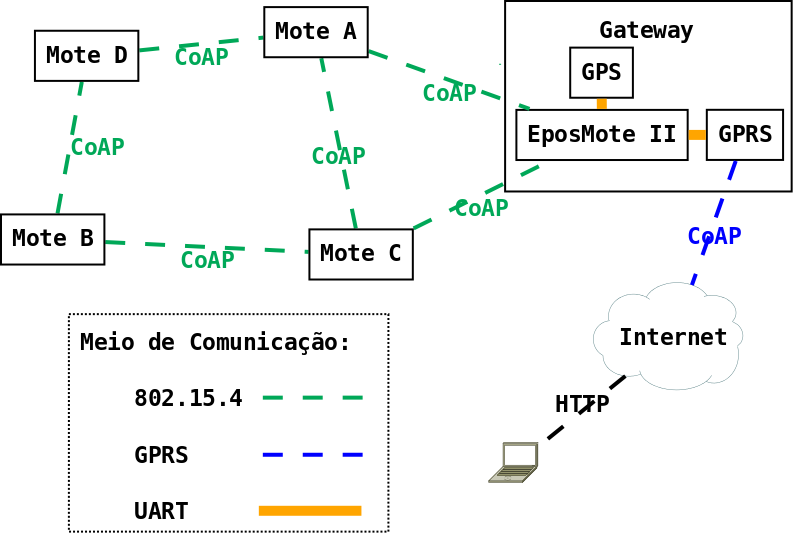
\includegraphics[width=0.9\linewidth]{../figuras/arquiteturaSlide}
\end{figure}
\end{frame}

\begin{frame}
\frametitle{Implementação}
\begin{itemize}
    \item Validação dos pacotes utilizando testes unitários, exemplos de outras bibliotecas, sniffing com Wireshark.
    \item A implementação do agendador de transmissão utiliza alarmes de disparo único.
    \item Exemplos de diveros recursos CoAP: coap:coap.me.
\end{itemize}
\end{frame}

%------------------------------------------------
\section{Avaliação}
%------------------------------------------------

\subsection{Ambiente de Testes}
\begin{frame}
\frametitle{Ambiente de Testes}
 \begin{table}[!ht]
  \centering
  \scriptsize
  \begin{tabular}{|c|p{3cm}|p{3cm}|}
	\hline
	& \textbf{contiki/client} & \textbf{epos/client}  \\ \hline
	\textbf{Microcontrolador}	  	  & Freescale MC13224V & Freescale MC13224V \\ \hline 
	\textbf{Plataforma Alvo}    & Econotag & EposMote II\\ \hline    
	\textbf{Sistema Operacional}    & Contiki & EPOS \\ \hline    
    \textbf{Ferramentas binárias}		  & GNU Binary Utilities (2.18.50-sg++) & arm-elf-binutils 4.4.4 \\ \hline
    \textbf{Compiladores}		  & GNU C \& C++ Compilers (4.3.2-sg++) & arm-elf-g++ 4.4.4\\ \hline
    \textbf{Bibliotecas C}          & Newlib C (1.16.0-sg++) & \\ \hline 
	\end{tabular}
  \end{table}
\end{frame}

\subsection{Resultados Experimentais}
\begin{frame}
\frametitle{Resultados Experimentais}

\begin{tikzpicture}
\centering
  \scriptsize
\label{memoryDiff}
\begin{axis}[ybar , enlargelimits =0.15, legend style ={ at ={(0.5,-0.15)}, anchor =north, legend columns =-1}, ylabel ={\# size in bytes}, symbolic x coords ={epos/cantcoap,contiki/minimal-net,contiki/erbium}, xtick =data, nodes near coords , nodes near coords align ={vertical},]
\addplot coordinates {(epos/cantcoap,62480) (contiki/minimal-net,59496) (contiki/erbium,62427)};
\addplot coordinates {(epos/cantcoap,216) (contiki/minimal-net,2432) (contiki/erbium,440)};
\addplot coordinates {(epos/cantcoap,10504) (contiki/minimal-net,22040) (contiki/erbium,18108)};
\addplot coordinates {(epos/cantcoap,73200) (contiki/minimal-net,83968) (contiki/erbium,81275)};
\legend {.text,.data,.bss, Total}
\end{axis}
\caption{Gr\'afico do tamanho das sess\~oes do arquivo ELF gerado para ARM.}
\end{tikzpicture}
\end{frame}

\section{Conclusão}

\subsection{Conclusões}
\begin{frame}
\frametitle{Conclusões}
\begin{itemize}
    \item Desenvolvimento de um gateway simplificado para redes de sensores sem fio e a Internet. 
    \item 
\end{itemize}
\end{frame}
\subsection{Trabalhos Futuros}
\begin{frame}
\frametitle{Trabalhos Futuros}

\begin{itemize}
    \item A implementa\c{c}\~ao da vers\~ao segura do protocolo CoAP, utilizando DLTS para comunica\c{c}\~ao segura entre os n\'os.
    \item Uma implementa\c{c}\~ao de servidor CoAP completa para executar utilizando a plataforma do EPOSMote II.

    \item Desenvolvimento de um gateway que utilize Software Defined Transceiver.

    \item Um gerador de c\'odigo que utiliza como entrada uma linguagem de especifica\c{c}\~ao dos recursos e a sa\'ida c\'odigo ANSI C m\'inimo de um servidor web utilizando CoAP e seus respectivos recursos.

    \item Modelo de apresentação de recursos para os usuários.
\end{itemize}
\end{frame}


%\begin{frame}
%\frametitle{Figure}
%Uncomment the code on this slide to include your own image from the same directory as the template .TeX file.
%%\begin{figure}
%%\includegraphics[width=0.8\linewidth]{test}
%%\end{figure}
%\end{frame}

%------------------------------------------------

%\begin{frame}[fragile] % Need to use the fragile option when verbatim is used in the slide
%\frametitle{Citation}
%An example of the \verb|\cite| command to cite within the presentation:\\~
%
%This statement requires citation \cite{p1}.
%\end{frame}

%------------------------------------------------

%\begin{frame}
%\frametitle{Bibliografia}
%\footnotesize{
%\begin{thebibliography}{99} % Beamer does not support BibTeX so references must be inserted manually as below
%\bibitem[Smith, 2012]{p1} John Smith (2012)
%\newblock Title of the publication
%\newblock \emph{Journal Name} 12(3), 45 -- 678.
%\end{thebibliography}
%}
%\end{frame}

%------------------------------------------------

\begin{frame}
\Huge{\centerline{Perguntas?}}
\end{frame}

%----------------------------------------------------------------------------------------

\end{document}
